\documentclass[12pt,a4paper]{article}
\usepackage[utf8]{inputenc}
\usepackage[T1]{fontenc}
\usepackage{times}                   % Font: Times New Roman
\usepackage[margin=2.54cm]{geometry} % Margins: 2.54cm
\usepackage{setspace}
\singlespacing                       % Line Spacing: Single Line
\usepackage{indentfirst}
\usepackage{graphicx}
\usepackage{float}
\usepackage{caption}
\usepackage{booktabs}
\usepackage{array}
\usepackage{multirow}
\usepackage{tabularx}
\usepackage{listings}
\usepackage{url}
\usepackage[numbers,sort&compress]{natbib}
\usepackage{hyperref}
\hypersetup{colorlinks=true,linkcolor=blue,citecolor=blue,urlcolor=blue}
\lstset{
    breaklines=true,
    breakatwhitespace=false,
    basicstyle=\ttfamily\footnotesize,
    frame=single,
    xleftmargin=1em,
    xrightmargin=1em
}
\newcolumntype{Y}{>{\raggedright\arraybackslash}X}

% Lightweight algorithm-style environment (no algorithmicx dependency)
\newcounter{algctr}
\newenvironment{procedure}[1]{%
  \par\medskip\noindent\refstepcounter{algctr}%
  \textbf{Procedure \thealgctr.} #1\par\nopagebreak
  \begin{enumerate}\setlength{\itemsep}{0pt}}{%
  \end{enumerate}\medskip}

\begin{document}

% =========================================================
% Cover Page
% =========================================================
\begin{titlepage}
    \centering
    \vspace*{2cm}
    {\Huge\bfseries 2nd Interim Report\par}
    \vspace{2cm}

    {\huge Towards Traceable Stablecoins in Decentralized Finance\par}
    \vspace{0.6cm}
    {\large An Evidence-Based Framework for Cross-Chain Stablecoin Traceability\par}

    \vfill

    {\large \textbf{Student Name:} Tang Tianhao\par}
    \vspace{0.5cm}
    {\large \textbf{Student Number:} 59720490\par}
    \vspace{1.5cm}
    {\large \textbf{Supervisor Name:} Prof LU Zhenliang\par}
    \vspace{0.5cm}
    {\large \textbf{Course:} CS6520 Project\par}
    \vspace{1.5cm}
\end{titlepage}

\newpage
\tableofcontents
\thispagestyle{empty}
\newpage
\clearpage
\setcounter{page}{1}

% =========================================================
\section*{Abstract}
\addcontentsline{toc}{section}{Abstract}
% =========================================================

Stablecoins have become a core settlement asset in decentralized finance (DeFi). Assets such as USDT and USDC combine price stability, deep liquidity, and cross-platform transferability, and are therefore widely used for DeFi trading, cross-border payment, exchange settlement, and on-chain arbitrage. The same properties, however, also make stablecoins an important vehicle for on-chain money laundering and financial crime. In particular, when cross-chain bridges, liquidity pools, mixers, and centralized exchanges all participate in a fund flow, the path of value is no longer a simple single-chain transfer graph, and traditional single-chain tracing methods struggle to explain where the funds are still traceable and where the trail has already been severed.

This project studies the traceability of stablecoin transactions in DeFi from a practical investigation angle. In this report, ``enhancing traceability'' means a limited but concrete task: after a transaction has already happened, I check how far the stablecoin path can be followed from public data. During implementation I found that a bridge name alone is not enough. A transaction may touch a known bridge contract, but that does not automatically reveal the recipient on the other chain. For this reason, the current system continues only when the next step is supported by a receipt, decoded event, calldata field, message identifier, or protocol status record. When that evidence is missing, the path is marked as unresolved rather than forced through amount or time similarity.

Compared with the first interim report, the work has moved from a broad AML-risk idea to a more specific tracing workflow. The main additions are: a graph representation for stablecoin fund paths; a comparison of ledger models and their tracing constraints; an evidence-based bridge classification; two reproduced bridge traces using real transactions (Across Ethereum-to-Arbitrum USDC and Stargate/LayerZero Ethereum-to-Arbitrum); one limited Solana CCTP~V2 parsing case; one limited Tron TRC-20 parsing case; and a clearer statement of where post-hoc tracing must stop, such as at mixers, exchange pools, maker-style bridges, or protocols without public one-to-one mappings.

% =========================================================
\section{Introduction}
% =========================================================

\subsection{Cryptocurrency Money Laundering at Scale}

Blockchain technology has lowered the barrier to transferring value globally. Compared with traditional financial systems, public-chain transactions are open, verifiable, permissionless, and cross-border. These properties have driven the growth of DeFi, stablecoins, on-chain exchanges, and cross-chain infrastructure, but they have also created new challenges for AML/CFT. An adversary can use anonymous or pseudonymous addresses, large numbers of relay wallets, DeFi protocols, and cross-chain bridges to move funds quickly, thereby increasing the cost of tracing.

Stablecoins sit at the center of this problem. Compared with volatile assets such as ETH or BTC, stablecoins can hold value on-chain over time without significant price fluctuation. For legitimate users, this makes stablecoins a convenient instrument for trading, payment, and settlement; for illicit funds, it also means that criminal proceeds can be moved quickly on-chain in a relatively stable value form. According to Chainalysis~\cite{chainalysis2024}, stablecoins have grown from a minor share to the majority of illicit on-chain transaction value, as criminals increasingly shift from Bitcoin toward stablecoins driven by their liquidity and ease of cross-chain transfer. Consequently, stablecoin traceability has become an important problem in on-chain compliance and DeFi security research.

Stablecoins differ fundamentally from generic crypto-assets such as BTC and ETH. BTC and ETH are closer to native on-chain assets, whose supply, transfer, and account state are governed primarily by base-layer protocol rules. Mainstream fiat-backed stablecoins such as USDT and USDC, by contrast, are typically issued as smart-contract tokens on public chains, and the issuer retains a contract-level control surface. The timing of this control matters: the issuer does not intervene in every ordinary peer-to-peer transfer. Issuer action concentrates in a few specific regimes --- \textbf{issuance} (minting against off-chain reserves), \textbf{redemption} (burning on redemption), \textbf{cross-chain migration} (burn-and-mint movement of supply between chains), and \textbf{risk enforcement} (freezing or blacklisting specific addresses). Circle's Cross-Chain Transfer Protocol (CCTP), for example, moves USDC across chains by burning on the source chain and minting to a recipient on the destination chain under issuer attestation, rather than by an ordinary token transfer~\cite{circleCCTP2026,circleCCTPTechnical2026}; Tether similarly mints and redeems USDT against reserves and has frozen specific addresses on request from authorities~\cite{tetherIssuancePrimer2024,tetherFreeze225m2023}. Fiat-backed stablecoins are therefore not entirely ``uncontrollable'' assets. They embed issuer governance, compliance enforcement, and account-control capability on top of an open blockchain, exercised at well-defined points rather than continuously.

This contract-level controllability is the reason I treat stablecoin tracing as a separate problem rather than as ordinary token analysis. If an issuer or exchange can freeze, reject, or flag an address, the decision should ideally be explainable: which upstream path caused the concern, which transaction records support that path, and where the public trail breaks. Without this explanation layer, the user only sees a black-box compliance result. In this sense, traceability sits between on-chain token control and off-chain compliance judgment.

The project therefore does not try to decide whether a given wallet is laundering money. Its question is narrower: when a stablecoin moves among addresses, contracts, bridges, exchanges, and DeFi protocols, which parts of the path can be verified from public evidence, which parts are only candidate leads, and which parts cannot be recovered after the fact?

\subsection{Cross-Chain Bridges and Regulatory Blind Spots}

Cross-chain bridges are critical infrastructure for DeFi fund flows. Users employ bridges to migrate assets among Ethereum, Arbitrum, Optimism, Base, Polygon, BSC, Linea, and other chains, in order to participate in the trading, lending, staking, and liquidity strategies of different ecosystems. However, cross-chain bridges also break the completeness of the single-chain transaction graph. Once funds leave the source chain, an analyst must determine whether they can still be traced on the destination chain.

Strictly speaking, one blockchain cannot directly ``transfer'' to another. A transaction on Ethereum cannot directly modify the ledger state of Linea, Arbitrum, or Tron. Even if assets on two chains represent the same economic unit, such as USDC or USDT, a decrease in the token balance on the source chain does not automatically cause an increase in the token balance on the destination chain. A cross-chain bridge enables asset migration because it establishes a protocol procedure between the two chains: it locks, burns, or escrows assets on the source chain, and releases, mints, or has a liquidity provider front the assets on the destination chain. The bridge is therefore a set of linked source-chain and destination-chain actions, not a single cross-chain transfer.

For cross-chain tracing, the task is not to find ``a single transaction that transfers directly from chain A to chain B,'' because such a transaction does not exist at the blockchain base layer. The real task is to check whether a \texttt{deposit}, \texttt{lock}, \texttt{burn}, or \texttt{message send} on the source chain can be connected, through public evidence, to a \texttt{mint}, \texttt{release}, \texttt{fill}, or \texttt{message execution} on the destination chain. This evidentiary connection may come from an event log, calldata, a message ID, a deposit ID, a sequence number, a VAA (Verified Action Approval, the signed cross-chain attestation used by Wormhole), or a protocol API, as reflected in public bridge and message-passing documentation~\cite{wormholeTokenTransfers2026,acrossApiDocs2026,layerzeroScanDocs2026}. Without such a connection, the code can only state that the user interacted with a certain bridge; it cannot claim to know the recipient on the destination chain.

Real-world on-chain laundering paths are often not simple single-chain multi-hop transfers. They combine multi-hop transfers, cross-chain bridges, liquidity pools, centralized exchanges, and privacy tools. Large attack events, such as fund flows related to the Ronin bridge, show that cross-chain movement has become part of complex value-transfer paths. I do not claim to reproduce the full Ronin path here. I use such cases as motivation: a tracing method that cannot explain what happens at a bridge is not enough for a real DeFi setting.

Public on-chain forensic reports have repeatedly documented adversaries combining chain hopping, bridges, and mixers for laundering~\cite{chainalysis2024,elliptic2023}. In the Ronin/Axie Infinity event, the stolen funds originated from the Ronin Bridge attack, after which the Lazarus Group used mixing services such as Tornado Cash and continued to move funds through cross-asset and cross-chain paths~\cite{chainalysisRonin2022,chainalysisTornado2022}. In the Harmony Horizon Bridge event, industry reporting indicates that the associated funds entered bridge protocols during later laundering stages and migrated between chains such as Bitcoin and Avalanche. These cases show that cross-chain bridges are not only targets of attack, but can also become part of post-attack fund washing and path complication.

I do not use these public attack cases as reproduced experiments. They are used only to motivate why bridge-aware tracing matters. For the actual experiments, I selected Across and Stargate/LayerZero transactions because their public records gave me enough fields to test the parser without relying on private labels. Across exposes a \texttt{V3FundsDeposited} event, a \texttt{depositId}, and an Across \texttt{/deposit/status} mapping. Stargate/LayerZero exposes message metadata, nonce, DVN verification, and a destination transaction. This separation is important: the public laundering cases explain \textit{why} the problem matters, while the two selected transactions show \textit{how} the current implementation resolves bridge links under two different mechanisms.

\subsection{Limitations of Existing Tools}

Existing tools and research exhibit four classes of limitations.

\textit{First}, commercial blockchain-analytics platforms typically have broad coverage, but their label provenance, cross-chain resolution rules, and risk-scoring methods are largely closed-source, making them difficult to reproduce and verify in an academic project.

\textit{Second}, many academic methods still take the single-chain transaction graph as their primary object. The Bitcoin UTXO model~\cite{weber2019} and the Ethereum account model have been studied extensively, but cross-chain bridges, liquidity pools, and multi-chain stablecoin flows have not been adequately handled in a way that explains each step of the path.

\textit{Third}, some cross-chain tracing methods rely on heuristic matching, such as similar amounts, close time windows, or the reuse of the same address across multiple EVM chains~\cite{mazorra2023}. Such methods can help surface candidate paths, but their evidentiary strength is insufficient to serve as a deterministic tracing conclusion.

\textit{Fourth}, stablecoin tracing requires integrating multiple kinds of evidence: ERC-20 Transfer logs, stablecoin issuer freeze lists, OFAC or other risk-address registries, bridge-contract registries, mixer labels, protocol APIs, and transaction receipts. In the absence of a unified traceability semantics, a system easily mislabels ``identified a bridge contract'' as ``already traced to the destination-chain address.''

Because of these limitations, I use a conservative rule in the implementation: continue tracing only when the transaction provides enough evidence to connect the next step. Otherwise, the result is kept as a possible lead, marked as unresolved, or stopped.

Commercial tools remain a useful reference. Public product descriptions of Chainalysis Reactor, for example, emphasize tracing swaps, bridges, DEXs, and mixers within a single investigation workflow and rendering complex contract activity into human-readable investigative steps~\cite{chainalysisReactor2026}. Chainalysis money-laundering reporting~\cite{chainalysis2024} also treats chain hopping via cross-chain bridges as one component of complex laundering strategies, particularly to describe how adversaries such as the Lazarus Group switch among mixers, bridges, and multi-chain environments. I borrow the ``follow the money across services'' investigative perspective, but I do not adopt black-box risk scoring as the core method. Instead, I break the problem into verifiable evidentiary questions: every cross-chain continuation must specify the source transaction, the bridge event, the message or deposit identifier, the destination transaction, and the evidence source.

\subsection{The Passive Taint Problem for Ordinary Users}

Ordinary users may, entirely unknowingly, receive stablecoins from a risk address or from an address downstream of a high-risk path. Exchanges and compliance systems may perform multi-hop backward tracing, and once the upstream of a user's received funds is close to a frozen address, a sanctioned address, a mixer, or a high-risk bridge, the user's account may be flagged. This phenomenon can be called the \textbf{passive taint problem}. Industry analysis has observed that a large fraction of blacklisted addresses had already moved their assets before the freeze took effect~\cite{blocksec2023}, which means tainted funds are already circulating among ordinary user addresses while those users remain unaware.

Passive taint shows that traceability is not only a problem for law enforcement, but also an important tool for ordinary users to understand the risk of their own funds. An interpretable system should explain which upstream address the risk comes from, how many hops away it is, at which protocol the path crosses chains, where the evidence lies, and where tracing stops. Otherwise, the user can only face a black-box risk score without understanding why they were flagged.

At this stage, passive taint is still a motivation and an interpretability target, not a completed quantitative module. A full treatment would need proportional flow accounting, otherwise a tiny contact with a risk path could be confused with the main source of the user's funds. I have not implemented that proportional model yet, so this report uses passive taint mainly to justify why the output should explain paths rather than only return a risk score.

\subsection{Research Objectives}

For this interim stage, I translated the broad objective of stablecoin traceability into four research questions:

\begin{enumerate}
    \item How can the stablecoin fund graph be formalized, distinguishing ordinary addresses, risk anchors, bridge destination nodes, unresolved protocol interactions, and stopping points?
    \item How can cross-chain bridge transactions be classified by traceability based on the \textit{evidence chain} rather than the bridge name?
    \item Can the current implementation, using public on-chain data, complete real source-chain to destination-chain bridge traces?
    \item When encountering new bridges, unregistered bridges, bridges without public one-to-one mappings, mixers, centralized exchanges, and pooled DeFi protocols, where must after-the-fact tracing stop?
\end{enumerate}

\subsection{Scope: Stablecoin Traceability and the Current EVM Focus}

The project title is broader than EVM stablecoins, so I discuss several ledger and execution models: UTXO, the EVM account model, Tron, Solana, centralized exchanges, and off-chain settlement systems. The implementation, however, still has a clear center of gravity. I pay most attention to fiat-backed stablecoins such as USDT and USDC because their contracts include issuer-side control functions, such as \texttt{mint}, \texttt{burn}, \texttt{freeze}, and \texttt{blacklist}. These functions make stablecoins different from native assets such as BTC or ETH, and they also make explanation more important when an address is restricted or treated as risky.

However, the implementation and experiments at this stage must bound their scope. The end-to-end bridge traces focus on EVM-like chains, because these chains share ERC-20 Transfer logs, smart-contract events, the \texttt{0x} address format, and Etherscan/Blockscout-style data interfaces. Non-EVM ecosystems such as Tron (TRC-20) and Solana (program/account model with SPL token accounts) require separate handling of their address formats, APIs, and transaction structure. As an initial step beyond EVM, this stage parses one real Solana and one real Tron transaction (Section~\ref{sec:nonevm}). These cases show that the data can be read and that the evidence format differs, but they are not presented as full end-to-end non-EVM bridge traces.

\subsection{Potential Outcome}

The expected deliverables of this stage include: a stablecoin tracing method based on explicit evidence; a way to classify bridge transactions by what they reveal; two real end-to-end bridge cases with different mechanisms (Across and Stargate/LayerZero); and an analysis of where after-the-fact tracing cannot continue.

% =========================================================
\section{Related Work}
% =========================================================

\subsection{Blockchain Transaction Graphs and AML Detection}

Blockchain AML research typically models transaction history as a graph, in which addresses or entities are nodes and transactions or fund flows are edges. Common methods include multi-hop neighbor search, taint propagation, transaction proximity, graph-based risk scoring, and graph neural networks~\cite{weber2019,bellei2024}. These methods provide a basis for on-chain fund tracing, but most study a single-chain environment.

Stablecoin tracing differs from native-asset tracing in a way that became obvious during the implementation. ERC-20 Transfer logs are useful because they let USDT and USDC movements be read separately from ETH native transfers. However, the raw address-to-address edge is often too literal. A transfer into a router, bridge, pool, vault, or exchange deposit address does not always mean that economic control has moved in the simple way suggested by the log. I therefore added protocol semantics and evidence strength on top of the basic transaction graph.

In addition, fiat-backed stablecoins carry an issuer-and-contract permission structure. Assets such as USDT and USDC can be minted, redeemed and burned, frozen, or blacklisted, unlike a decentralized-issuer asset such as BTC. Existing freeze and blacklist mechanisms show that stablecoin risk governance is no longer a purely off-chain compliance judgment, but contract behavior that can directly affect on-chain token state. For this reason, stablecoin tracing cannot stop at the level of ``there is a transfer between addresses,'' but must explain why a given address is flagged, how the fund path connects to a risk anchor, and what on-chain evidence underlies any control action taken by an issuer or platform.

\subsection{Cross-Chain Transaction Tracing and Traceability}

Cross-chain tracing research seeks to connect a \texttt{deposit}, \texttt{lock}, \texttt{burn}, or \texttt{message send} on the source chain with a \texttt{mint}, \texttt{release}, \texttt{fill}, or \texttt{execution} on the destination chain. Some methods use amount similarity, time windows, and same-address-control assumptions for matching~\cite{mazorra2023,sun2025track}. Such methods can broaden coverage, but this project does not treat them as deterministic evidence. A recent survey~\cite{ren2025survey} identifies cross-chain tracing as the area most lacking systematic study.

My bridge-related work focuses on \textbf{bridge detection and source-to-destination mapping}. In practice, I check whether the protocol exposes fields such as \texttt{destinationChainId}, \texttt{recipient}, \texttt{depositId}, \texttt{transferId}, \texttt{messageId}, \texttt{nonce}, \texttt{sequence}, a VAA, or a source-tx-to-destination-tx mapping. If these fields are present and can be verified, tracing can continue. If they are absent, the output should say that the path is uncertain or broken. Sun et al.~\cite{sun2025track} make a similar observation: transparency varies dramatically across bridges, with message-passing protocols sometimes exposing counterpart transaction hashes through APIs, while liquidity-pool bridges often make the direct input--output relationship unavailable.

\subsection{Multi-Hop Risk Scoring and Tree-Based Tracing}

Multi-hop risk scoring typically starts from a target address, expands upstream or downstream along the transaction graph, and computes risk according to distance from a risk anchor. The earliest formalization of propagating risk from known illicit addresses, with \textit{Poison} and \textit{Haircut} propagation, dates to M\"{o}ser et al.~\cite{moser2014}; TaintRank~\cite{hercog2019} later analogized taint propagation to PageRank. From the opposite direction, Circle's \textit{Transaction Proximity}~\cite{liao2025} measures distance from \emph{legitimate} anchors over the whole Ethereum graph. Fixed-depth BFS is simple and intuitive, but may be too shallow against deliberately constructed laundering paths, and too deep for ordinary users and high-frequency contracts, causing false positives and computational blow-up.

I retain adaptive-depth BFS and hop decay, but I use them as tracing tools rather than as final risk labels. The BFS output should be a fund-path tree with evidence source, distance decay, and break type, not a simple list of ``bad'' addresses.

\subsection{Machine Learning for Stablecoin AML}

A separate line of work applies machine learning to stablecoin AML, using features such as transaction frequency, in/out degree, amount distribution, interaction counterparties, and temporal patterns to identify anomalous addresses; the most comprehensive stablecoin-specific study to date trains tree ensembles over thousands of labeled addresses~\cite{juvinski2026}. These classifiers are useful for prioritizing suspicious wallets, but they need labels and a much larger dataset than this interim project has. More importantly, a classifier score does not by itself explain a fund path. For that reason, I did not make a machine-learning classifier the core contribution in this stage. I instead focused on whether each step in a traced path has an explicit on-chain or protocol evidence source.

\subsection{Regulatory Frameworks}

The FATF Travel Rule~\cite{fatf2023}, the EU regulatory regime~\cite{euaiact2024}, stablecoin issuer freeze mechanisms, and on-chain sanctions lists together form the compliance backdrop of stablecoins. Regulatory rules emphasize that virtual-asset service providers identify and report risky transactions, but in DeFi a large amount of activity occurs among non-custodial wallets, smart contracts, and cross-chain bridges. Public research must distinguish on-chain evidence, external labels, and data returned by protocol APIs, and avoid disguising private labels or black-box scores as verifiable conclusions.

\subsection{Interpretability and Privacy-Preserving Compliance}

Interpretability is an important requirement of this project. A traceability system should explain why a path exists, where its evidence comes from, how a cross-chain link is confirmed, and why tracing cannot continue at certain points.

Privacy-preserving compliance is a related direction. Auditable privacy pools~\cite{buterin2023} let users prove that their funds belong to a compliant set, or do not belong to a known illicit set, without revealing the full transaction history. However, proof-of-innocence approaches depend on the completeness and timeliness of blocklists~\cite{constantinides2025}, and empirical work on Tornado Cash sanctions shows that legal and technical enforcement around privacy protocols remains difficult~\cite{brownworth2024}: a deposit flagged as illicit after passing the check has already entered the pool irreversibly. When after-the-fact tracing stops at a mixer, a bridge without public one-to-one mappings, or a privacy protocol, protocol-level compliance becomes relevant. I discuss this only as background, not as a current implementation target.

\subsection{Summary}

In summary, existing work provides transaction-graph analysis, multi-hop risk scoring, cross-chain matching, and AML classification tools. My route in this stage is narrower: for each step of a stablecoin path, I ask what evidence supports it, and I stop when that evidence is not available.

% =========================================================
\section{System Modeling and Structure}
% =========================================================

\subsection{Architecture Overview}

The current implementation can be read as two layers.

The first layer is fund-path analysis. It builds the fund graph from stablecoin Transfer logs and labels ordinary addresses, contract addresses, risk anchors, bridge contracts, mixers, unresolved protocol interactions, and points where tracing must stop.

The second layer checks the evidence behind each step. This is where most of the bridge work sits: after a source-chain bridge interaction is detected, the code tries to prove whether it can be connected to a destination chain, destination address, or destination transaction. The Across and Stargate cases were chosen to test this layer rather than to make claims about those particular users.

Internally, these two layers are realized by separable components, shown in Figure~\ref{fig:system_architecture}: per-chain data clients and bridge-specific parsers feed the analysis engine, which consults risk-address lists and emits structured report objects. Keeping these components separate is what allows a new chain or bridge to be added by extending a client or parser rather than rewriting the engine.

\begin{figure}[H]
    \centering
    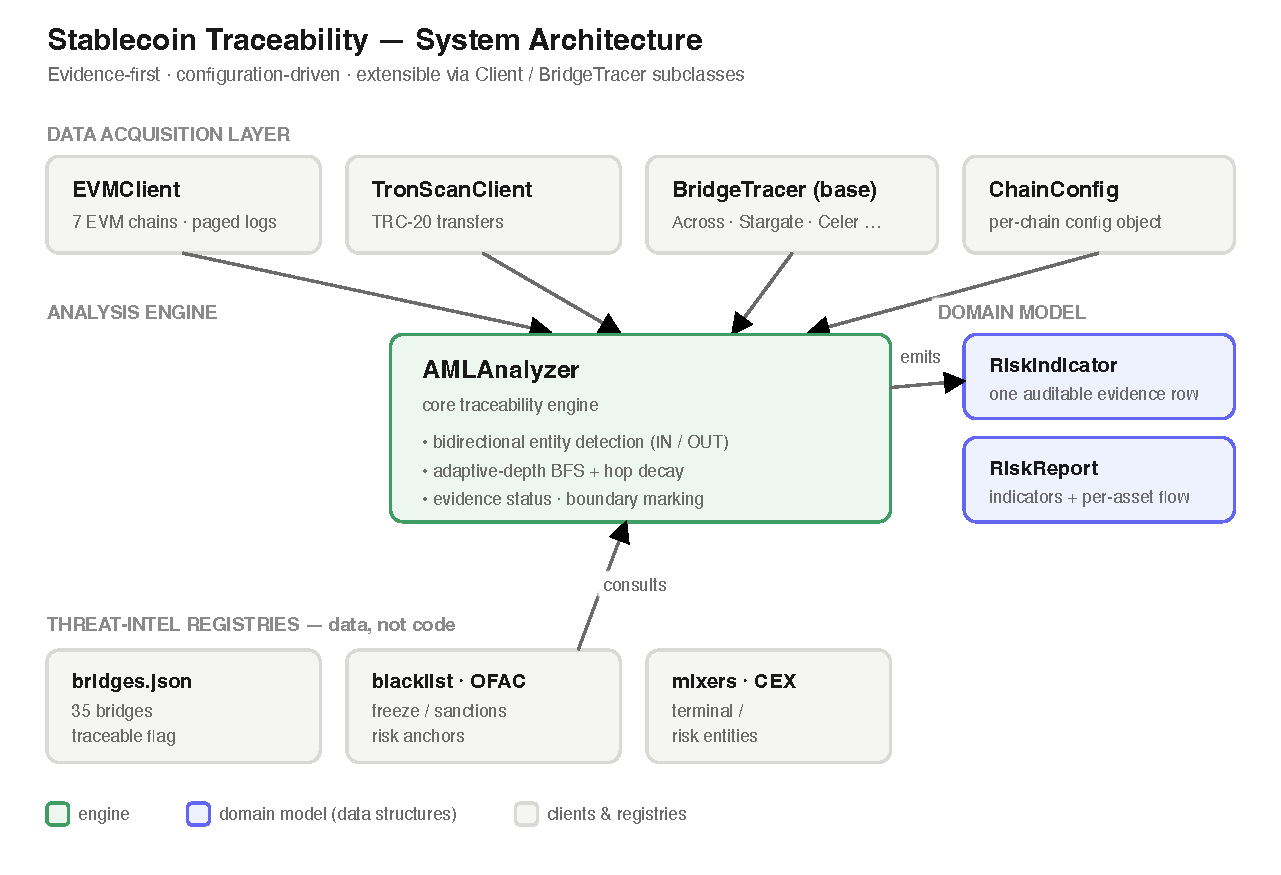
\includegraphics[width=\textwidth]{figures/stablecoin_traceability_architecture_v2.pdf}
    \caption{System architecture of the stablecoin tracing implementation. The analyzer is separated from chain clients, bridge parsers, risk-address lists, and report data structures.}
    \label{fig:system_architecture}
\end{figure}

\subsection{Design Choices and Justifications}

The core design choice is simple but restrictive: continue only when there is evidence. For ordinary stablecoin transfers, I rely on ERC-20 Transfer logs. For cross-chain bridges, I use event logs, calldata, a \texttt{depositId}, a \texttt{messageId}, or a protocol API. For risk anchors, I use a blacklist, freeze list, or sanctions list. For unknown bridges and protocols that do not reveal one-to-one relationships, the output records that tracing cannot be completed from public data.

This design is more conservative than heuristic methods, but better suited to the academic goal of this project. It can clearly answer: what we know, where the evidence is, where we still do not know, and where it is theoretically impossible to recover the path from public on-chain data.

% =========================================================
\section{Methodology and Algorithms}
% =========================================================

\subsection{Traceability Formalization}

The stablecoin fund graph is represented as a directed graph $G = (V, E)$. The node set $V$ includes ordinary addresses, contract addresses, risk anchors, bridge destination nodes, unresolved protocol interactions, and stopping points. The edge set $E$ represents stablecoin transfers, cross-chain bridge results, or mappings supplied by a protocol API.

Each edge must carry evidence metadata, including chain, token, amount, transaction hash, timestamp, event type, log index, and resolution method. Based on the evidence source, this project distinguishes the following types.

\begin{table}[htbp]
\centering
\caption{Evidence used by the stablecoin tracing graph.}
\label{tab:evidence_types}
\small
\begin{tabularx}{\textwidth}{l l Y}
\toprule
\textbf{Evidence type} & \textbf{Source} & \textbf{Meaning} \\
\midrule
token transfer & ERC-20 Transfer log & A stablecoin transfer occurred between two addresses. \\
on-chain protocol data & event log / calldata & The protocol exposes the destination chain, destination address, or message identifier. \\
official API or explorer & official API / explorer & A protocol indexer provides a source-to-destination mapping. \\
external label & blacklist / risk-address list & The address or contract is flagged by an external source. \\
heuristic lead & time / amount similarity & Usable only for candidate discovery, not as deterministic evidence. \\
\bottomrule
\end{tabularx}
\end{table}

\subsection{Accounting Models and Tracing Constraints}
\label{sec:accounting}

Traceability is not a property that is naturally uniform across all blockchains; it depends on the ledger model and on what transaction data, message identifiers, and protocol metadata are publicly observable. Table~\ref{tab:accounting} summarizes this comparison. The key observation is that the difficulty of tracing is determined less by the chain ``name'' than by how a given accounting model is \emph{used} by DeFi primitives.

\begin{table}[htbp]
\centering
\caption{Accounting models and their tracing constraints.}
\label{tab:accounting}
\small
\begin{tabularx}{\textwidth}{l Y Y}
\toprule
\textbf{System type} & \textbf{Observable tracing data} & \textbf{Main limitation} \\
\midrule
Bitcoin / UTXO & input--output coin lineage & Weakly connected to the DeFi stablecoin contract ecosystem. \\
EVM fiat-backed stablecoins & ERC-20 logs, mint/burn events, freeze/blacklist state, contract events & Contract intermediaries, routers, and pools change economic semantics. \\
Native crypto-assets (e.g., ETH) & native transfers and transaction traces & Lacks a stablecoin issuer control surface. \\
Tron / TRC-20 & TRC-20 transfer records (account model, similar to EVM) & Address format and APIs differ and require separate adaptation. \\
Solana & token accounts and program invocations & Different program/account model. \\
CEX / custody & deposit and withdrawal addresses & Internal ledger is invisible. \\
Mixer / privacy protocol & intentionally hidden input--output relation & After-the-fact tracing stops at this protocol. \\
\bottomrule
\end{tabularx}
\end{table}

For this reason, I discuss the general stablecoin-tracing problem across several systems, but I keep the completed experiments mainly on EVM-like chains. This is a scope decision for the second-stage implementation, not a change of the overall topic.

For EVM fiat-backed stablecoins, traceability has an additional meaning. Since the token contract may support \texttt{mint}, \texttt{burn}, \texttt{freeze}, or \texttt{blacklist}, there is already an on-chain governance interface. The tracing layer should help explain that governance: if an address is treated as risky, the report should show which risk anchor it connects to, which transactions and events support the path, and whether the path still survives a bridge or DeFi interaction.

\subsection{Bridge Registry and Evidence-Based Classification}

A cross-chain bridge is not just one contract address. In the traces I inspected, a single bridging flow can involve a source contract, a destination contract, a message layer, a relayer, a liquidity pool, or a market maker. Therefore, I do not judge traceability by the bridge name alone. I judge whether this specific transaction reveals enough information to connect the source side with the destination side.

It is also important to distinguish a bridge from a relayer. A bridge is the whole cross-chain protocol or system: source-chain contracts, destination-chain contracts, message verification, liquidity pools, settlement rules, and often an API or explorer. A relayer is only one participant in that system. It may submit a message on the destination chain, or it may front liquidity to the user before being repaid by the protocol. In an Across-style liquidity/relayer-fill model, the source-chain deposit and the destination-chain payment are not the same on-chain transfer. The destination payment is an independent fill by a relayer or liquidity system. Therefore, tracing must connect the two through protocol evidence such as a \texttt{depositId}, message identifier, fill transaction, or official status API.

Several specific bridge protocols are referred to throughout this report. Because their designs differ in ways that directly affect traceability, Table~\ref{tab:bridge_who} briefly introduces each one before the analysis proceeds.

\begin{table}[htbp]
\centering
\caption{Cross-chain bridge protocols referenced in this report.}
\label{tab:bridge_who}
\small
\begin{tabularx}{\textwidth}{l l Y}
\toprule
\textbf{Protocol} & \textbf{Type} & \textbf{One-line description} \\
\midrule
Across & liquidity/relayer-fill bridge & A relayer fronts the asset on the destination chain against the user's source-chain deposit; the protocol's status API maps a deposit to its fill transaction. \\
Stargate & message-passing bridge (on LayerZero) & A unified-liquidity bridge that sends a cross-chain message through the LayerZero messaging layer; delivery is indexed by LayerZero Scan. \\
LayerZero & generic messaging layer & Not a token bridge itself, but the message-passing infrastructure (endpoints, message GUID, DVN verifiers) that Stargate and others build on. \\
Celer cBridge & lock-and-release liquidity bridge & Locks funds on the source chain and releases pooled liquidity on the destination chain, linked by a \texttt{transferId}. \\
Wormhole & message-passing bridge & Emits a signed attestation (a VAA) that the destination chain verifies before releasing or minting the asset. \\
Axelar / Squid & message-passing bridge \& router & Axelar provides cross-chain messaging; Squid is a router built on top of it for swaps and transfers. \\
Orbiter & maker/solver bridge & A market maker fills the user on the destination chain, with no public one-to-one on-chain link between the two legs. \\
Synapse & pooled-liquidity bridge & Funds enter and leave a shared liquidity pool, so the input--output correspondence is not individually identifiable. \\
Rollup official bridges & canonical lock-and-mint & The native deposit bridges of L2 rollups (e.g., Arbitrum, Optimism), where the same user address is typically preserved on the L2. \\
\bottomrule
\end{tabularx}
\end{table}

In principle, a cross-chain bridge solves the problem of ``how two ledgers that do not share state can express the same asset migration.'' Since chain A cannot write directly to chain B, bridge protocols typically adopt one of several mechanisms, summarized in Table~\ref{tab:bridge_mech}.

\begin{table}[htbp]
\centering
\caption{Cross-chain bridge mechanisms and their traceability implications.}
\label{tab:bridge_mech}
\small
\begin{tabularx}{\textwidth}{l Y Y Y}
\toprule
\textbf{Bridge mechanism} & \textbf{Source-chain action} & \textbf{Destination-chain action} & \textbf{Traceability implication} \\
\midrule
lock-and-mint & lock source asset & mint wrapped asset & Must prove lock corresponds to mint. \\
burn-and-mint & burn source token & mint token & Must prove burn message corresponds to mint. \\
lock-and-release & lock or escrow on source & release existing liquidity & Must prove release stems from the same bridge request. \\
liquidity/relayer fill & user pays on source & relayer or LP fronts on destination & Needs depositId/fillTx or API proof. \\
message-passing bridge & send message on source & execute message on destination & Needs messageId/nonce/sequence/VAA. \\
\bottomrule
\end{tabularx}
\end{table}

All of these mechanisms create at least two records: one on the source chain and another on the destination side. The bridge may connect them through a message layer, validators, a relayer, a liquidity provider, or an official indexer. My tracing logic therefore does not pretend that there is one physical cross-chain transfer edge. It looks for the evidence that proves both records belong to the same bridge action.

Cross-chain bridges also have inherent shortcomings. \textit{First}, different bridges have no unified standard interface. Across, LayerZero, Wormhole, Axelar, Celer, Stargate, and official rollup bridges expose different fields and APIs, so the tracing system must implement separate parsing logic for different bridges. \textit{Second}, the security assumptions of bridges are complex and may depend on validator sets, light clients, multisigs, relayers, oracles, or liquidity providers; once a bridge is attacked, its ``cross-chain representation'' may diverge from the real collateral. \textit{Third}, under liquidity-bridge and maker/solver models, the destination-chain payment may be fronted by a third party, so there need not be a simple one-to-one on-chain transfer edge between the source user and the destination recipient. \textit{Fourth}, new bridges can be deployed at any time and may not immediately have public labels, documentation, or APIs. \textit{Fifth}, some bridges or aggregators may deliberately reduce public information, making tracing difficult at the protocol level.

These shortcomings changed how I define ``traceable.'' I do not assume that all bridges can be traced through. A bridge is useful for deterministic tracing only if the protocol exposes a usable relationship between the source-chain action and the destination-chain action. Fields such as \texttt{destinationChainId}, \texttt{recipient}, \texttt{messageId}, \texttt{depositId}, \texttt{sequence}, a VAA, or a source-to-destination transaction mapping strengthen the link. If the public data only shows pooled funds entering and leaving, or a maker fronting payment without a one-to-one relationship, the result should remain a lead or become a stopping point.

The current implementation uses a manually curated bridge-contract list to recognize known bridge interactions. I treat this list as a helper, not as ground truth. Anyone can deploy a new bridge-like contract, and many contracts are not well documented. For an unregistered or unverified bridge, the code does not guess the destination-chain path. Based on this practical limitation, I classify bridge interactions into five categories (Table~\ref{tab:bridge_class}).

\begin{table}[htbp]
\centering
\caption{Evidence-based bridge interaction categories.}
\label{tab:bridge_class}
\small
\begin{tabularx}{\textwidth}{l Y Y}
\toprule
\textbf{Category} & \textbf{Meaning} & \textbf{Trace action} \\
\midrule
directly parseable bridge & event/call data directly exposes destination chain and recipient & continue tracing \\
bridge requiring official API & official API or explorer provides the destination transaction & continue tracing, while recording API dependence \\
contract identified only & known bridge contract, but the current transaction does not resolve the destination address & keep as a possible lead \\
unresolved protocol interaction & possibly a new bridge or complex protocol, but without sufficient public information & stop and mark unresolved \\
stopping point & bridge without one-to-one mapping, mixer, exchange pool, privacy protocol & stop deterministic tracing \\
\bottomrule
\end{tabularx}
\end{table}

\subsection{Cross-Chain Resolution Workflow}

The core goal of cross-chain resolution is to decide whether a source-chain transaction can be connected to a destination-chain execution. Common fields include:

\begin{itemize}
    \item \texttt{destinationChainId} or \texttt{dstChainId};
    \item \texttt{recipient}, \texttt{receiver}, \texttt{toAddress};
    \item \texttt{depositId}, \texttt{transferId}, \texttt{messageId}, \texttt{nonce}, \texttt{sequence}, \texttt{VAA};
    \item a source-to-destination transaction mapping returned by an official API.
\end{itemize}

The resolution flow is given in Procedure~1 below.

\begin{procedure}{Evidence-first cross-chain bridge resolution.}
\item Identify whether the stablecoin transaction involves a known bridge contract.
\item Fetch the source-chain transaction receipt.
\item Decode event logs and calldata.
\item Extract destination chain, destination address, and cross-chain message identifier.
\item If necessary, call the protocol API or explorer.
\item Fetch the destination-chain transaction receipt.
\item If the relationship is verifiable, add a destination-chain node and continue tracing.
\item Otherwise, keep the path as a possible lead or stop tracing.
\end{procedure}

This flow can be understood as three layers. The first is \textbf{protocol identification}: judging whether a counterparty is a known bridge or bridge-related contract. The second is \textbf{evidence verification}: checking whether this specific transaction contains verifiable cross-chain evidence, such as a destination chain ID, recipient, \texttt{depositId}, or \texttt{messageId}. The third is \textbf{trace continuation}: switching to the destination chain when evidence is sufficient, and stopping with a marked status when it is not.

The bridge list only answers ``what protocol this might be,'' not ``where the money went.'' What decides continuation is the evidence inside this transaction and the related protocol records. For a liquidity/relayer-fill model such as Across, the source-chain transaction is a deposit event on Ethereum, while the asset received on Arbitrum is filled later by a relayer or liquidity system. My tracing logic connects those two records through the \texttt{depositId} and the Across \texttt{/deposit/status} API. It traces the relationship exposed by the bridge protocol, not a non-existent direct inter-chain transfer.

\subsection{Adaptive-Depth BFS and Hop Decay}

Within a single chain, I use BFS to expand the stablecoin fund graph. Hop decay expresses how risk or contamination strength decreases with distance. It cannot create evidence by itself; it only describes distance over a path that already has evidence.

For ordinary paths I keep a smaller tracing depth. For paths close to a risk anchor or bridge interaction, I retain more evidence information because those are exactly the places where a later explanation may be needed. This is a compromise between coverage and false positives.

% =========================================================
\section{Preliminary Analysis}
% =========================================================

This section records what I have actually tested so far. The central task is to reconstruct a stablecoin path across a bridge using verifiable evidence only. I use two real bridge traces (Sections~\ref{sec:across} and~\ref{sec:stargate}) because they cover different bridge mechanisms and different protocol indexers. I then compare the current bridge coverage, add two small non-EVM parsing checks, and state where the current method stops.

\subsection{Across Ethereum-to-Arbitrum USDC Bridge Trace}
\label{sec:across}

The first case is a real Across Protocol V3 USDC transfer from Ethereum to Arbitrum. I used it to check whether the cross-chain resolution workflow could move from a source-chain deposit event to a destination-chain fill transaction.

The sample is a reproducible technical case selected from public on-chain data, not a laundering case. I first queried \texttt{V3FundsDeposited} events from the Across V3 SpokePool contract on Ethereum, then filtered for USDC/USDT transfers. I kept a transfer only if the event fields were complete, the Across status API returned \texttt{filled}, and the destination-chain receipt could still be queried. This selection rule matters because the purpose is to test bridge resolution, not to make a risk judgment about the address.

The source transaction is

\begin{lstlisting}
0x024b2b3cfffddb12ef9b93da592f1ec754c457281b11be4e24324cd26359b3f5
\end{lstlisting}

The source chain is Ethereum and the bridge protocol is Across Protocol V3. The code first obtains the source-chain transaction receipt via the Etherscan V2 API and locates the \texttt{V3FundsDeposited} event. The decoded fields are shown in Table~\ref{tab:across_src}.

\begin{table}[htbp]
\centering
\caption{Decoded source-chain \texttt{V3FundsDeposited} event from the project experiment record.}
\label{tab:across_src}
\small
\begin{tabularx}{\textwidth}{l Y}
\toprule
\textbf{Field} & \textbf{Value} \\
\midrule
depositId & 1502687 \\
destination chain & Arbitrum \\
destination chain ID & 42161 \\
depositor & \texttt{0xcb9055fc2a8f0f27041dc238574100a22df0c15e} \\
recipient & \texttt{0xcb9055fc2a8f0f27041dc238574100a22df0c15e} \\
input amount & 40{,}000.012359 USDC \\
output amount & 39{,}996.803276 USDC on Arbitrum \\
\bottomrule
\end{tabularx}
\end{table}

The next step cannot be recovered from the Ethereum receipt alone. I then call the Across \texttt{/deposit/status} API and query the bridge status by source transaction and \texttt{originChainId + depositId}~\cite{acrossApiDocs2026}. The API returns the fields in Table~\ref{tab:across_status}.

\begin{table}[htbp]
\centering
\caption{Across \texttt{/deposit/status} API response from the project experiment record.}
\label{tab:across_status}
\small
\begin{tabularx}{\textwidth}{l Y}
\toprule
\textbf{Field} & \textbf{Value} \\
\midrule
status & filled \\
destination fill tx & \texttt{0x5f81158cdd5c0ea56c50c6ddbea411e1a08ca031c56fcf057cddc60b0c1cd7ee} \\
destination chain ID & 42161 \\
\bottomrule
\end{tabularx}
\end{table}

Finally, the returned fill transaction is checked again on Arbitrum through the Etherscan V2 multi-chain API. This last step is important because I do not want the API response alone to be treated as the final proof.

This case is traceable, but only with a clear caveat: the middle step depends on the Across API. The implementation does more than identify an Across contract, because it also finds the destination-chain fill transaction. However, the bridge link is not inferred from amount or time-window similarity. It is based on the source-chain event, the \texttt{depositId}, and the protocol status API.

The evidence strength is not uniform across the three steps, so I separate it explicitly into source-chain receipt, protocol indexer, and destination-chain receipt.

\begin{enumerate}
    \item \textbf{Source step.} The \texttt{V3FundsDeposited} event is read directly from the Ethereum transaction receipt and decoded by us. Its correctness depends only on the integrity of the Ethereum ledger, not on any third party. This yields the \texttt{depositId}, destination chain ID, and recipient.
    \item \textbf{Bridge-indexer step.} The mapping from \texttt{depositId} to the destination \texttt{fillTx} is \emph{not} something we can derive from the source chain alone, because the fill is an independent transaction that a relayer submits later on Arbitrum, and no source-chain field points to it. We obtain this mapping by querying the Across \texttt{/deposit/status} indexer. Its correctness depends on the honesty and availability of the Across indexer, and is strictly weaker than on-chain self-evidence. If the API were discontinued or returned incorrect data, this link could not be independently reconstructed from public logs.
    \item \textbf{Destination step.} We do not take the API response at face value. We use the returned \texttt{fillTx} hash to fetch the actual transaction receipt on Arbitrum and confirm that the transaction exists on-chain. This re-anchors the indexer result back to verifiable ledger data.
\end{enumerate}

The externally indexed step is therefore checked on both sides against on-chain receipts. This distinction matters. If the destination address is encoded directly in source-chain calldata, the evidence is mostly on-chain. In this Across case, the destination transaction is found through a status API, so the result depends on the protocol indexer. The report output should preserve that difference instead of presenting both cases as equally strong.

\subsection{Stargate / LayerZero Message-Passing Bridge Trace}
\label{sec:stargate}

One Across example is not enough to show that the method works beyond one protocol. I therefore ran a second case on Stargate, which uses LayerZero message passing rather than the Across liquidity/relayer-fill model. This also changes the evidence source: Across uses the Across \texttt{/deposit/status} API, while Stargate relies on LayerZero Scan to index the cross-chain message.

The source transaction
\begin{lstlisting}
0x5955c3c28ee325ae6570793afd7ffb6c4b8416543f4695c739db95b7455485a1
\end{lstlisting}
on Ethereum was confirmed to interact with a known LayerZero endpoint. After that, LayerZero Scan returned the message record and delivery status on the destination chain. The parsed result is summarized in Table~\ref{tab:stargate}.

\begin{table}[htbp]
\centering
\caption{Stargate / LayerZero cross-chain message from the project experiment record.}
\label{tab:stargate}
\small
\begin{tabularx}{\textwidth}{l Y}
\toprule
\textbf{Field} & \textbf{Value} \\
\midrule
bridge family & Stargate (message-passing via LayerZero) \\
source chain & Ethereum (srcEid 30101) \\
destination chain & Arbitrum (dstEid 30110) \\
message GUID & \texttt{0xcc519912...450c14} \\
nonce & 82123 \\
LayerZero status & DELIVERED (executor transaction confirmed) \\
DVN verification & 3 required DVNs: LayerZero Labs, Nethermind, Canary (all SUCCEEDED) \\
destination tx & \texttt{0xc4740664...91cfd16} (receipt observed on Arbitrum) \\
\bottomrule
\end{tabularx}
\end{table}

The evidence chain has the same broad shape as Across: source-chain receipt, protocol indexer, and destination-chain receipt. The details are different enough to be useful. First, the middle step is served by LayerZero Scan rather than the Across API, so the workflow is not tied to one protocol's tooling~\cite{layerzeroScanDocs2026}. Second, the message-passing model exposes more verification metadata. The LayerZero record includes a GUID, a nonce, and a Decentralized Verifier Network (DVN) attestation set. In this case, the three required DVNs (LayerZero Labs, Nethermind, Canary) all reported \texttt{SUCCEEDED}. I then fetched the destination transaction receipt on Arbitrum to re-anchor the indexed result on-chain. With Across and Stargate both resolved end-to-end, the current workflow has been tested on two bridge mechanisms rather than a single special case.

\subsection{How Different Bridges Are Currently Handled}
\label{sec:bridgesurface}

The two traces above cover two bridge mechanisms, but they do not mean the system has broad bridge coverage. Table~\ref{tab:bridge_surface} records the current state more conservatively. It separates bridges that have been traced from source chain to destination chain, bridges for which I only have partial parsing code, bridges that are only recognized by contract address, and bridges whose design does not publish a one-to-one source-to-destination relationship.

\begin{table}[htbp]
\centering
\caption{How different bridge families are currently handled.}
\label{tab:bridge_surface}
\scriptsize
\begin{tabularx}{\textwidth}{l l Y l}
\toprule
\textbf{Bridge} & \textbf{Mechanism} & \textbf{Connection evidence} & \textbf{Status} \\
\midrule
Across V3 & liquidity fill & deposit event + \texttt{depositId} + status API & completed case \\
Stargate & LayerZero message & endpoint + LayerZero Scan message record & completed case \\
Celer cBridge & lock/release & \texttt{Send} event + cBridge API & code only \\
Rollup official & canonical bridge & deposit event; same \texttt{0x} user on L2 & recognized only \\
Orbiter / Synapse & pooled/maker fill & no public one-to-one mapping & stop \\
\bottomrule
\end{tabularx}
\end{table}

Two points follow from this table. First, each bridge needs its own parsing method. Across and Stargate both require an official or protocol-related indexer for the final hop: Across status API for the fill transaction, and LayerZero Scan for the delivered message. A rollup canonical bridge may sometimes be checked more directly from events and the same user address on the L2. Second, the status column is deliberately literal. Across and Stargate have real transactions and saved results. Celer has parsing code but no completed experiment. Rollup official bridges are recognized by contract address in the current code. Orbiter and Synapse-style pooled or maker flows do not publish a one-to-one relationship, so I do not claim a destination address for them.

\subsection{Non-EVM Surfaces: Initial Parsing of Solana and Tron}
\label{sec:nonevm}

Both end-to-end bridge cases above are on EVM chains. To avoid treating EVM as the whole stablecoin world, I also ran two small parsing checks outside EVM: one real Solana transaction and one real Tron transaction. These are intentionally not presented as full bridge traces. They only test whether the chain's native data format can be read and whether stablecoin-relevant evidence can be extracted. Table~\ref{tab:nonevm} summarizes what each case established.

\begin{table}[htbp]
\centering
\caption{Initial non-EVM parsing cases from the project experiment records.}
\label{tab:nonevm}
\small
\begin{tabularx}{\textwidth}{l Y l}
\toprule
\textbf{Chain} & \textbf{What was parsed and verified} & \textbf{Level reached} \\
\midrule
Solana & A real transaction decoded via Solana JSON-RPC; identified two Circle CCTP~V2 programs (\texttt{MessageTransmitter}, \texttt{TokenMessengerMinter}), the \texttt{ReceiveMessage} / \texttt{HandleReceiveUnfinalizedMessage} instructions, and a confirmed SPL USDC balance change. & bridge program identified \\
Tron & A real TRC-20 transaction read via TronGrid/TronScan; confirmed one USDT token transfer with sender, receiver, and amount. & token-level transfer evidence \\
\bottomrule
\end{tabularx}
\end{table}

The contrast with the EVM cases is the main result here. On Solana, the parser identifies the cross-chain program and the USDC movement, but I do not infer a destination chain because that would require recovering the CCTP message nonce and querying Circle's attestation service. On Tron, the account model is closer to EVM at the token-transfer level, so TRC-20 sender, receiver, and amount are easier to read. Bridge-side tracing on Tron still needs separate handling. In short, Solana and Tron have been reached at the parsing level, not at the end-to-end bridge-tracing level.

\subsection{Fundamental Limits of Post-hoc Tracing}
\label{sec:limits}

A public blockchain does not make every fund path traceable. After-the-fact tracing depends on whether the protocol exposes enough information. From the current experiments and code review, I identify the following limits:

\begin{enumerate}
    \item \textbf{New or unregistered bridges}: a contract may actually perform cross-chain functions, but without a public label, documentation, or stable event format.
    \item \textbf{Bridges without one-to-one public mappings}: a maker, solver, or pooled-liquidity model may show funds entering and leaving pools without revealing the direct relationship between the source user and the destination recipient.
    \item \textbf{Mixers or privacy protocols}: the purpose of the protocol is precisely to sever the input--output relationship.
    \item \textbf{Centralized exchanges or custody pools}: the chain shows only deposits and withdrawals; the internal ledger is invisible.
    \item \textbf{DeFi pooling}: AMMs, vaults, lending pools, and aggregators may mix funds as part of normal business logic.
\end{enumerate}

At these points, the implementation should not turn a guess into a deterministic path. It either keeps the result as a possible lead or stops tracing.

This also clarifies the difference between this work and commercial on-chain analytics platforms. Tools such as Chainalysis can combine on-chain data, service labels, OSINT, proprietary clustering, and investigation workflows. Public materials indicate that Chainalysis Reactor emphasizes integrated tracing across multiple chains, assets, bridges, DEXs, and mixers~\cite{chainalysisReactor2026}, and its money-laundering reporting~\cite{chainalysis2024} treats bridges and mixers as important parts of complex laundering paths. My project does not have those private labels or clustering tools. Instead, I choose a narrower goal that can be checked in an academic setting: within public on-chain data and public protocol metadata, show which cross-chain paths have evidence, which are only leads, and which must stop.

% =========================================================
\section{Milestones and Overall Schedule}
% =========================================================

This section explains what has changed since the first interim report. The first report mainly built the foundation: why stablecoins matter for on-chain laundering and compliance, how ordinary users may receive risky funds without knowing it, and why bridges, mixers, exchanges, and regulations matter. On the code side, I already had an early address-analysis program, some stablecoin transfer records, and an initial way to describe risky addresses through transfer counts, sender/receiver relationships, and amount distributions. That stage answered why the problem matters and what on-chain data could be used.

In this second report, I narrowed the topic from broad AML detection to stablecoin path explanation. This is not just a wording change. A risk score alone does not tell a user or analyst where the risk came from. If funds cross a bridge, a score also does not explain where the funds arrived on the other chain. The current report therefore focuses on evidence for each path step. If the evidence is not enough, the trace should stop instead of being forced through amount or timing similarity.

The first-stage data and code are not discarded; I reorganized them. The stablecoin transfer records, blacklisted addresses, bridge contract list, mixer and exchange labels, and rule-engine logic are now used to decide whether a fund path has public evidence behind it. The earlier transparent/opaque bridge distinction is also more concrete now. Some bridges write destination chain and recipient into events; some require an official API to find the destination transaction; some can only be recognized as bridge interactions; and some bridges, mixers, or exchange pools do not publish one-to-one relationships at all. The goal is to reduce guessing and make clear why a path can or cannot be followed.

Experimentally, the most important progress is two real bridge cases. In the Across case, I start from a USDC bridge transaction on Ethereum, read the \texttt{depositId}, destination chain, and recipient from the Across event, query the Across status API for the Arbitrum fill transaction, and then check that the Arbitrum transaction exists. In the Stargate/LayerZero case, I follow a message-passing flow where LayerZero Scan provides the message GUID, nonce, verification status, and destination transaction. Together, these cases show that the implementation has been run on two different bridge mechanisms instead of only one custom example.

The current stage also includes Solana and Tron, but the claim is deliberately limited. The Solana CCTP case is not a full bridge trace. It shows that the relevant evidence is program instructions, account lists, and SPL token balance changes, not ERC-20 events. The Tron USDT case is also not a full bridge trace. It shows that a TRC-20 transfer can be read with sender, receiver, and amount, while bridge or exchange-side movement still needs separate handling. These two cases show that the data formats can be parsed, not that full non-EVM bridge coverage is complete.

Overall, the second stage moves the project from a general AML risk tool toward a system that explains how far stablecoin funds can be followed. The first report supplied the background, early code, and data materials. This report turns them into a more testable route: define what evidence can support a path, distinguish bridges that can and cannot be parsed, validate the method with Across and Stargate, and state where tracing must stop.

% =========================================================
\section{Work to be Completed for the Next Report}
% =========================================================

For the final report, the main task is to combine the first-stage risk-scoring work with the second-stage bridge-tracing work into one complete system. The first interim report focused on adaptive-depth BFS, hop-decay risk scoring, blacklist proximity, and passive-taint analysis. This second interim report focuses on evidence-based stablecoin traceability, especially whether a bridge transaction can be continued from the source chain to the destination chain. The final system should connect these two parts: trace the fund path first, then calculate and explain the risk based on the evidence found along that path.

First, I need to integrate the BFS layer with the bridge-resolution layer. At present, single-chain BFS can expand from a target address and identify nearby risk anchors such as blacklist addresses, mixers, and suspicious relays. The bridge parser can separately decide whether a cross-chain transaction is traceable, unresolved, or a stopping point. In the next version, these two components should work in the same trace tree. A traceable bridge should allow the BFS search to continue on the destination chain, while an opaque bridge, mixer-like bridge, centralized exchange, or pooled protocol should become a marked terminal node.

Second, the risk-scoring logic should be revised so that it uses evidence status, not only hop distance. The first-stage system used hop decay to reduce risk with distance from a blacklist or other risk anchor. This is still useful, but the final version should also distinguish different evidence strengths. A path supported by direct on-chain receipts is stronger than a path that depends on a protocol indexer, and both are stronger than a heuristic lead. If a bridge does not expose a one-to-one mapping, the system should not assign the same confidence as a fully resolved bridge trace.

Third, the bridge experiments should be expanded carefully. Across and Stargate/LayerZero are completed cases, but they are still only two examples. The next step should be to add one or two representative bridges only if their evidence fields are clear enough to evaluate. Bridges should be classified by auditability and traceability: directly parseable, API-assisted, contract-identified only, unresolved, or deterministic stopping point. The report should avoid describing bridge operators as simply good or bad; the more useful distinction is whether a specific bridge interaction exposes enough public evidence for tracing.

Finally, the output should become more user-facing and auditable. A final risk report should include the numerical risk score, the evidence chain, the bridge-resolution status, the source and destination transactions when available, and the reason tracing stops when evidence is insufficient. This is especially important for the passive-taint scenario discussed in the first report: ordinary users need to understand not only that an address may be risky, but also where the risk came from and how reliable that conclusion is.

% =========================================================
\addcontentsline{toc}{section}{References}
\bibliographystyle{ieeetr}
\bibliography{sample}

\end{document}
